\section{\SeeDB Execution Engine}
\label{sec:optimizer}
\mpv{Short intro based on S3}

\subsection{Basic Implementation}
\label{sec:basic_implementation}

In the basic implementation of \SeeDB, for each aggregate view, \SeeDB generates
a SQL query corresponding to the target
and reference view, and issues
the two queries, one at a time, to the database.
It repeats this process for each aggregate view stub.
As the results are received, \SeeDB can compute the
distance between the target and comparison view
distributions, and identify the $k$ visualizations
with highest utility. 

Naturally, this basic implementation has many inefficiencies.
In a table with $a$ dimensions, $m$ measures, and $f$ aggregation functions, 
$2\times f \times a \times  m$ queries must be executed independently.  
As we show in Section~\ref{sec:experiments}, this can >100s for
large data sets (with hundreds of attributes and millions of rows).
These latencies are unacceptable for interactive use.
In this paper, we propose two different suites of optimizations to deal with these
inefficiencies.
The first type of optimizations, discussed in Section~\ref{sec:sharing_opt}, involve work {\em sharing},
i.e., combining view-computation queries as much as possible.
The second type of optimizations, discussed in Section~\ref{sec:in_memory_execution_engine}, involve {\em pruning}, where some aggregate views are not completely evaluated over the whole data set.
 The second suite of optimizations
are approximate, in that they, since they use utility estimates, there is a small likelihood that the returned visualizations may not have the highest utility.

%!TEX root=document.tex
\section{{\large \SeeDB\ } Execution Engine}
The goals of the \SeeDB execution engine are to efficiently
compute the utility of a large number of aggregate views
and to then find and display the $k$ visualizations with the highest utility.

\subsection{Basic Implementation} \label{sec:dbms-exec-engine}

We now describe the basic implementation of \SeeDB
over a traditional relational database system.
Recall that the input to the \SeeDB engine is a set of 
aggregate view stubs, i.e., triples of the form
$(a, m, f)$, where $a$ is the dimension attribute, $m$ is the measure,
and $f$ is the aggregation function.
For each aggregate view stub, we craft
a SQL query corresponding to the target
and comparison view, and issue
the two queries, one at a time, to the database.
We then repeat this for each aggregate view stub.
As the results are obtained, we can compute the
distance between the target and comparison view
distributions, and keep track of the $k$ visualizations
with highest utility. These are then displayed
to the analyst.


Naturally, this basic implementation has many inefficiencies.
In a table with $a$ dimensions, $m$ measures, and $f$ aggregation functions, 
$2\times f \times a \times  m$ queries must be executed independently.  
As we show in Section~\ref{sec:experiments}, this can take minutes in
large data sets (with hundreds of attributes and millions of rows), which is too long for interactive use. \mpv{are we at interactive time scales?}
We propose two different suites of optimizations to deal with these
inefficiencies.
The first suite of optimizations, discussed in Section~\ref{sec:sharing-opt}, concerns {\em sharing}, \mpv{grouping sets are the other end of sharing}
i.e., sharing as much work as possible while leveraging the 
backend database system.
The second suite of optimizations, discussed in Section~\ref{sec:in_memory_execution_engine}, concerns {\em pruning},
i.e., avoiding the complete computation of some aggregate views
by pruning them away. The second suite of optimizations
are approximate, in that they, since they use utility estimates, there is a small likelihood that the returned visualizations may not have the highest utility.
%  in rare occasions may lead
% to inaccurate results (in that the visualizations
% displayed need not be the ones with the best utilities).

% Our first instantiation of the \SeeDB\ engine uses SQL queries in a
% traditional database system to evaluate the utility of each view.
% %We explore this design because it enables \SeeDB\ to be easily integrated 
% %with visualization systems that use DBMSs for data storage (e.g. Tableau, 
% %Spotfire etc).
% The advantage of this design is that it benefits
% from all the features of a standard relational engine and can be easily integrated into systems
% that use DBMSs for data storage.
% However, the efficiency of this approach is somewhat limit because
% the only way to interact with data is via SQL queries.
% %On the downside, this design limits \SeeDB\ to using the API
% %exposed by the DBMS; essentially, 
% %\SeeDB\ can only open/close connections to the
% %database and execute one or more SQL queries. 
% %Since we have no control over how queries are executed or access to intermediate
% %results, 

% Given a set of view stubs provided to the execution engine, conceptually,
% the basic approach proceeds as follows:
% (1) for each view, we generate SQL queries for the target and
% comparison view---recall that these are aggregate queries, where
% the target view is the aggregate query corresponding 
% to the visualization being considered, and the comparison
% view is the aggregate query that is being compared against,
% for the purpose of utility computation;
% see Section \ref{sec:problem_statement}, 
% (2) we execute each view query independently on the DBMS, 
% (3) the results of each query (i.e. the aggregated values) are processed and
% normalized to compute the target and comparison distributions, 
% (4) we compute utility for each view 
% and select the top-$k$ views with the largest utility,
% which are then sent to the frontend.
% This strawman approach is clearly inefficient since it examines every possible view and 
% executes each view query independently.

\subsection{Sharing-Based Optimizations}\label{sec:sharing-opt}
In this section, we focus on minimizing total execution time
by reducing the
total number of queries issued to the database,
and by reducing the total number of scans of the underlying table.
Specifically, we apply the following optimizations:
\agp{I didn't make a smoothing pass on the rest of this..}

\stitle{Combine Multiple Aggregates}: All aggregate view queries 
with the same group-by attribute can be 
rewritten as a single, combined query. So instead of executing
queries for views $(a_1$, $m_1$, $f_1)$, $(a_1$, $m_2$, $f_2)$ \ldots $(a_1$, $m_k$, $f_k)$
independently, we combine them into a single view represented by
$(a_1, \{m_1, m_2\ldots m_k\}$, $\{f_1, f_2\ldots f_k\})$.  We have found that there is no penalty
to grouping as many aggregates as possible in both row and column stores. 

\stitle{Combine target and comparison view query}:
Since the target view and comparison views only differ in the subset of data
that the query is executed on, we rewrite these two view queries as
one. For instance, the target and comparison view queries $Q1$ and $Q2$
shown below, can be combined into a single query $Q3$.
\vspace{-5pt}
\begin{align*} 
Q1 = &{\tt SELECT \ } a, f(m) \ \ {\tt FROM} \  D\  {\tt WHERE \ \ x\ <\ 10\
GROUP \ \ BY} \ a \\
Q2 = &{\tt SELECT \ } a, f(m) \ \ {\tt FROM} \  D\  {\tt GROUP \ \ BY} \ a \\
Q3 = &{\tt SELECT \ } a, f(m), {\tt CASE\ IF\ x\ <\ 10\ THEN\ 1\ ELSE\ 0\
END}\\ 
&as\ g1,\ 1\ as\ g2 \ \ {\tt FROM} \ D\ {\tt GROUP \ \ BY} \ a,\ g1,\ g2
\end{align*}

\stitle {Parallel Query Execution}:
  We execute multiple view queries in parallel since we expect co-executing queries 
  to share buffer pool pages and reduce disk accesses times. 
  However, the precise number of parallel queries needs to be tuned to take into account 
  buffer pool contention, locking and cache line contention \cite{Postgres_wiki}. 
  %As a result, we must identify the optimal number of parallel queries for our workload.

% We can do much better if we can use a single scan to evaluate multiple views simultaneously.

% In fact, our ideal operator $\mathcal{O}$ would perform a single scan of the
% data and compute all query results in one pass to return the top-$k$ views.
% Current database systems do not support this functionality.
% A handful of systems have recently introduced the SQL GROUPING
% SETS\footnote{GROUPING SETS allow the simultaneous grouping of query results by
% multiple sets of attributes.} functionality that could be used to support this
% operation. However, the grouping sets operator will not scale to tables with 
% a large number of attributes due to the large size of intermediate results.
% size of the eventual result maintained in memory will be $2 \times a \times f
% \times m$ attributes, multiplied by the size of an aggregate distribution.
% Furthermore, as we show in Section \ref{sec:in_memory_execution_engine},
% evaluating all views for the entire dataset is unnecessary and inefficient. 
% We can achieve much better performance by aggressively pruning low-utility
% views on the fly.

% Without this ideal operator $\mathcal{O}$,
% our optimizations minimize table scans in two ways: (1) minimize the total number of
% queries by intelligently combining queries, and (2) reduce the total
% execution time by running queries in parallel. 
% Our DBMS-backed execution engine for \SeeDB\ is agnostic towards the
% particular DBMS used to execute queries.
% However, because of significant differences in the way that row stores and
% column stores organize data, some of the optimizations described below
% will be more powerful in row stores and may actually hurt performance in column
% stores. In our experimental evaluation (Section \ref{sec:experiments}), we study
% the relative advantages of each of our optimizations for row and column stores.
% The optimizations supported by \SeeDB\ are described below.

% \subsubsection {Combine Multiple Aggregates} 
% A large number of view queries have the same group-by attribute but different
% aggregation attributes. 
% Therefore, \SeeDB\ combines all view queries with the same
% group-by attribute into a single, combined view query. For instance, instead of executing
% queries for views $(a_1$, $m_1$, $f_1)$, $(a_1$, $m_2$, $f_2)$ \ldots $(a_1$, $m_k$, $f_k)$
% independently, we can combine the $n$ views into a single view represented by
% $(a_1, \{m_1, m_2\ldots m_k\}$, $\{f_1, f_2\ldots f_k\})$. We demonstrate later
% on (Section \ref{sec:expts_dbms_execution_engine})  that this optimization
% offers a speed-up roughly proportional to the number of measure attributes.

\stitle {Combine Multiple Group-bys}:
% Efficient cube materialization is a problem well studied in the OLAP literature.
% Since the views considered by \SeeDB\ can be thought of as projections of the OLAP
% cube, we can adapt efficient materialization techniques to our problem.
After applying our multiple aggregate optimization, we are left with a number of 
queries with a group-by on a single aggregate.
We can of course group these together into a single query, but but each additional 
group by attribute will increase the number of groups, and (possibly) lead to slower
overall performance when the number of groups becomes large.  
Therefore, \SeeDB\ has to determine the optimal way of executing these multi-attribute
{\it group-by} queries.
%Savvy readers will recognize this problem as being a special case of materializing
%an OLAP cube~\cite{olap_cube}.
%Views evaluated by \SeeDB\ are projections of the OLAP cube and we can adapt techniqes
%from the cube literature~\cite{} to find the optimial execution strategy for these queries.
% There are few differences in the \SeeDB\ setting and traditional OLAP cubes: (1) OLAP
% cube materialization is performed inside the database giving more flexibility in the
% techniques used; in \SeeDB\ every evaluation corresponds to a separate query; (2) 
%Specifically, we work with a similar problem formulation: 
Our specific problem is as follows: given a space budget $\mathcal{S}$,
and estimates of sizes of views (i.e. number of rows in the result), we need to the optimal
way to combine multiple single-attribute group-by queries into multi-attribute group-by queries.
If we know the number of distinct values for each attribute, we can estimate the
size of a view containing dimension attributes $a_i$ and $a_j$ as $|a_i|\times |a_j|$.
Formally, our problem becomes:
\vspace{-5pt}
\begin{problem}[Optimal Grouping]
Given a set of dimension attributes $A$ = \{$a_1$\ldots$a_n$\}, divide the
dimension attributes in $A$ into groups $A_1, \ldots, A_l$ (where $A_i$ is some
subset of $A$ and $\bigcap A_i$=$A$) such that if a query $Q$ groups the table by $A_i$, 
the total space budget for $Q$ does not exceed $\mathcal{S}$.
\vspace{-5pt}
\end{problem}

Notice that the above problem is isomorphic to the NP-Hard {\em bin-packing} problem~\cite{garey}.
If we let each dimension attribute
$a_i$ correspond to an item in the bin-packing problem with weight $\log (|a_i|)$,
and set the bin size to be $\log \mathcal{S}$,
then packing items into bins is identical to finding groups $A_1, \ldots, A_l$,
such that the estimated size of any query result is below $\mathcal{S}$.
We use the standard first-fit algorithm~\cite{first-fit} to find the optimal
grouping of dimension attributes.

\agp{get rid of this para if we are describing in related work. This problem is superficially similar to the problem of OLAP cube materialization~\cite{olap_cube}, where
the goal is to pre-compute aggregates across some dimensions of a dataset to optimize cube queries,
subject to a total space budget and given a historical workload.  The problem, however, is actually quite different:
we have a set of aggregates we {\it must} compute as efficiently as possible, whereas in the cube materialization
literature the goal is to pre-compute a part of the cube subject to a space bound, without concern for how long the 
(offline) pre-computation takes.}

% The first-fit algorithm works as follows:
% on initialization, all groups $A_1, \ldots, $ $A_l$ are empty.
%   For each dimension attribute, considered in an arbitrary order, place it in the first group
%   $A_i$ that it can ``fit into'', i.e., the worst case
%   number of distinct values for that $A_i < \tau$.
%   For bin-packing, this algorithm has a guarantee of using up to 1.7X more 
%   bins than necessary: here, this translates to up to 1.7X more groups than necessary.
% Notice that since this grouping is independent of the input query, we can
% perform grouping offline using more computationally expensive techniques as
% well.


% since we now store the aggregate for every combination
% of $a_1, a_2, \ldots, a_n$, 
% the number of aggregates that need to be recorded 
% is the number of distinct combinations
% of $(a_1, \ldots, a_n)$, which, in the worst case, 
% is proportional to $\prod_i |a_i|$.
% Thus, the number of aggregates that need to be recorded 
% grows exponentially (in the worst case) in the
% number of group-by attributes. 
% We will show (Section \ref{sec:experiments}) that 
% the time to execute a query with multiple group-by attributes does indeed
% depend on the number of distinct values present in the 
% combination of dimension attributes. 
% From a DBMS perspective, this is expected because keeping track of a large
% number of aggregates impacts computational time (e.g. for sorting in sort-based aggregate)
% as well as temporary storage requirements (e.g. for hashing in hash-based
% aggregate) making this technique ineffective for large numbers of
% distinct values.

% Consequently, when we combine group-by attributes, we must ensure that the
% number of distinct values remains {\it small enough}, below a specific 
% threshold $\tau$, that we determine based on system parameters.
% For simplicity, we ignore the correlations between dimension attribute values,
% and work with worst-case estimates. 
% The upper limit on the number of distinct values for a given combination of
% group-by attributes is given by the product of the number of distinct values
% for each attribute.
% For example, if we combine three dimension attributes $a_i$, $a_j$ and $a_k$
% with $|a_i|$, $|a_j|$ and $|a_k|$ distinct values respectively, the maximum number of
% distinct groups is $|a_i|\times |a_j| \times |a_k|$.
 % The number of distinct groups in turn depends on the correlation between
 % values of attributes that are being grouped together. 
 % For instance, if two
 % dimension attributes $a_i$ and $a_j$ have $n_i$ and $n_j$ distinct values
 % respectively and a correlation coefficient of $c$, the number of distinct
 % groups when grouping by both $a_i$ and $a_j$ can be approximated by
 % $n_i$$\ast$$n_j$$\ast$(1-$c$) for $c$$\neq$1 and $n_i$ for $c$=1 ($n_i$ must
 % be equal to $n_j$ in this case).
  
% Therefore, our problem can be stated as follows:
% \begin{problem}[Optimal Grouping Optimization]
% Given a set of dimension attributes $A$ = \{$a_1$\ldots$a_n$\}, divide the
% dimension attributes in $A$ into groups $A_1, \ldots, A_l$ (where $A_i$ is some
% subset of $A$ and $\bigcap A_i$=$A$) such that the worst-case number of distinct values
% for each group is below $\tau$.
% \vspace{-5pt}
% \end{problem}

\stitle{Other Optimizations}: 
To further speedup processing, we can pre-compute results for 
static views (e.g. comparison views on full tables) or operate on
pre-computed data samples.  Such optimizations are orthogonal to the
problem of efficiently evaluating a large number of views, which we will have to
do even in the presence of pre-computaiton or sampling, so we don't focus on them here.

In the experimental evaluation, we show that the optimizations described in this section can lead to speedups of XXX.
The absolute latency numbers are in the interactive range for small and medium datasets, but we find that for larger datasets latency falls in the 50-150 range which is unacceptable for an interactive system.
In the next section, we discuss a few techniques that allow us to reliably prune out  views what will have low utility. 

%do not address the more important challenge of evaluating a large number of views.

%In Section \ref{XXX} we show that this optimization gives us a speedup of XXX.

% Given that the problem is NP-Hard, we use two strategies to group dimension attributes;
% the first strategy is adapted from the standard first-fit approximation algorithm~\cite{first-fit}
% for bin-packing; the second strategy is adapted from Huffman coding~\cite{huffman-codes}.
  
% \squishlist
% \item {\bf First-Fit}: The algorithm is simple;
% at first, all groups $A_1, \ldots, $ $A_l$ are empty.
% For each dimension attribute, considered in an arbitrary order, place it in the first group
% $A_i$ that it can ``fit into'', i.e., the worst case
% number of distinct values for that $A_i < \tau$.
% For bin-packing, this algorithm has a guarantee of using up to 1.7X more
% bins than necessary: here, this translates to up to 1.7X more groups than necessary.
  % In this trategy, we set an upper limit $V$ on the
  % number of distinct groups that any combination of dimension attributes can
  % produce.
  % Now, suppose that each dimension attribute $a_i$ $\in A$ has $n_i$ distinct
  % values.
  % We cast the problem of finding the optimal grouping of dimension attributes as
  % a version of bin-packing.
  % Let each dimension attribute $a_i$ be an item with volume $log(n_i)$ and
  % suppose that we are given bins of volume $log(V)$.
  % Then finding the optimal grouping of attributes is exactly equivalent to
  % finding the optimal packing of attribute items into the minimum number of
  % bins.
%   \item {\bf Huffman-Grouping}: Here, the algorithm works as follows:
%   we start by assigning each dimension attribute its own group,
%   and maintain these groups in sorted ascending order.
%   At each step, we take the two smallest groups out of this sorted list, combine
%   the dimension attributes in both of them into one new group, and then
%   add this new group to the mix and re-sort.
%   We keep doing this until we cannot combine the two smallest groups any more
%   without violating the threshold $\tau$.
% \squishend
% If this was vanilla bin-packing, the first-fit algorithm would be sufficient to
% find near-optimal groupings. 
% The advantage of having the huffman-grouping algorithm is the following: Instead
% of having a hard threshold $\tau$ on the worst-case number of distinct groups,
% the huffman-grouping algorithm can also adapt to the case where we
% are instead provided a black-box function that, given a particular
% grouping of attributes, returns a value for the ``goodness'' of the combination.
% As we will see in Section~\ref{sec:analytical_model}, 
% we develop an analytical model for the performance (i.e., the execution time)
% of the DBMS-backed execution engine. 
% This model can be used to derive this black-box function.
% Given a black-box function, the huffman-grouping algorithm operates
% as follows: until the ``goodness'' of the grouping keeps increasing 
% (i.e., the predicted execution time keeps decreasing),
% repeatedly combine the two smallest groups into a single group.
% We experimentally evaluate both strategies in Section \ref{sec:experiments}.
% 
% \srm{In 6.2.2., we mention the model.    Are we keeping this?  I think it could be ok to put the details in the appendix if we can show one graph that illustrates that the model can be used to predict how many groups to choose, etc.}

% \subsubsection{Combine target and comparison view query}
% \label{subsec:target_comparison_view}
% Since the target view and comparison views only differ in the subset of data
% that the query is executed on, we can easily rewrite these two view queries as
% one. For instance, for the target and comparison view queries $Q1$ and $Q2$
% shown below, we can add a group by clause to combine the two queries into $Q3$.
% \begin{align*} 
% Q1 = &{\tt SELECT \ } a, f(m) \ \ {\tt FROM} \  D\  {\tt WHERE \ \ x\ <\ 10\
% GROUP \ \ BY} \ a \\
% Q2 = &{\tt SELECT \ } a, f(m) \ \ {\tt FROM} \  D\  {\tt GROUP \ \ BY} \ a \\
% Q3 = &{\tt SELECT \ } a, f(m), {\tt CASE\ IF\ x\ <\ 10\ THEN\ 1\ ELSE\ 0\
% END}\\ 
% &as\ g1,\ 1\ as\ g2 \ \ {\tt FROM} \ D\ {\tt GROUP \ \ BY} \ a,\ g1,\ g2
% \end{align*}
% This rewriting allows us to obtain results for both queries in a single table
% scan. The impact of this optimization depends on the selectivity of the
% input query and the presence of indexes. When the input query is less selective,
% the query executor must do more work if the two queries are run separately. In
% contrast, in the presence of an index, running selective queries independently
% may be faster.
% \srm{In 4.2.3., I don't understand why the combined query wouldn't always be faster.  It seems like you are replacing two scans with one, which should just be better.  How could it not be (unless there are very selective filter predicates that aren't show in the example???)}
% \agp{I agree.}

% \subsubsection {Combine Multiple Group-bys}
% \label{subsec:mult_gb}
%   Similar to the multiple aggregates optimization, another optimization
%   supported by \SeeDB\ is to combine multiple queries with different group-by
%   attributes into a single query with multiple group-by attributes.
%   For instance, instead of executing queries for views $(a_1$, $m_1$, $f_1)$,
%   $(a_2$, $m_1$, $f_1)$ \ldots $(a_n$, $m_1$, $f_1)$ independently, we can
%   combine the $n$ views into a single view represented by $(\{a_1, a_2\ldots
%   a_n\}$, $m_1$, $f_1)$ and post-process results.

% Unlike the previous optimization, where the speed-up is proportional to the
% number of view queries combined, in this case, the situation is not as straightforward. 
% The reason for this is the following:
% since we now store the aggregate for every combination
% of $a_1, a_2, \ldots, a_n$, 
% the number of aggregates that need to be recorded 
% is the number of distinct combinations
% of $(a_1, \ldots, a_n)$, which, in the worst case, 
% is proportional to $\prod_i |a_i|$.
% Thus, the number of aggregates that need to be recorded 
% grows exponentially (in the worst case) in the
% number of group-by attributes. 
% We will show (Section \ref{sec:experiments}) that 
% the time to execute a query with multiple group-by attributes does indeed
% depend on the number of distinct values present in the 
% combination of dimension attributes. 
% From a DBMS perspective, this is expected because keeping track of a large
% number of aggregates impacts computational time (e.g. for sorting in sort-based aggregate)
% as well as temporary storage requirements (e.g. for hashing in hash-based
% aggregate) making this technique ineffective for large numbers of
% distinct values.

% Consequently, when we combine group-by attributes, we must ensure that the
% number of distinct values remains {\it small enough}, below a specific 
% threshold $\tau$, that we determine based on system parameters.
% For simplicity, we ignore the correlations between dimension attribute values,
% and work with worst-case estimates. 
% The upper limit on the number of distinct values for a given combination of
% group-by attributes is given by the product of the number of distinct values
% for each attribute.
% For example, if we combine three dimension attributes $a_i$, $a_j$ and $a_k$
% with $|a_i|$, $|a_j|$ and $|a_k|$ distinct values respectively, the maximum number of
% distinct groups is $|a_i|\times |a_j| \times |a_k|$.
%  % The number of distinct groups in turn depends on the correlation between
%  % values of attributes that are being grouped together. 
%  % For instance, if two
%  % dimension attributes $a_i$ and $a_j$ have $n_i$ and $n_j$ distinct values
%  % respectively and a correlation coefficient of $c$, the number of distinct
%  % groups when grouping by both $a_i$ and $a_j$ can be approximated by
%  % $n_i$$\ast$$n_j$$\ast$(1-$c$) for $c$$\neq$1 and $n_i$ for $c$=1 ($n_i$ must
%  % be equal to $n_j$ in this case).
  
% Therefore, our problem can be stated as follows:
% \begin{problem}[Optimal Grouping Optimization]
% Given a set of dimension attributes $A$ = \{$a_1$\ldots$a_n$\}, divide the
% dimension attributes in $A$ into groups $A_1, \ldots, A_l$ (where $A_i$ is some
% subset of $A$ and $\bigcap A_i$=$A$) such that the worst-case number of distinct values
% for each group is below $\tau$.
% \vspace{-5pt}
% \end{problem}
% Notice that the problem as stated above is isomorphic to the NP-Hard
% {\em bin-packing} problem~\cite{garey}: to see this, we let each dimension attribute
% $a_i$ correspond to an item in the bin-packing problem with weight $\log (|a_i|)$,
% and we set the threshold on the bin size to be $\log \tau$,
% then packing items into bins is identical to finding groups $A_1, \ldots, A_l$,
% such that the worst-case number of distinct values is below $\tau$.
% Thus, the problem as stated above is NP-Hard.

% We use the standard first-fit algorithm~\cite{first-fit} to find the optimal
% grouping of dimension attributes.
% The first-fit algorithm works as follows:
% on initialization, all groups $A_1, \ldots, $ $A_l$ are empty.
%   For each dimension attribute, considered in an arbitrary order, place it in the first group
%   $A_i$ that it can ``fit into'', i.e., the worst case
%   number of distinct values for that $A_i < \tau$.
%   For bin-packing, this algorithm has a guarantee of using up to 1.7X more 
%   bins than necessary: here, this translates to up to 1.7X more groups than necessary.
% Notice that since this grouping is independent of the input query, we can
% perform grouping offline using more computationally expensive techniques as
% well.

  % \subsubsection {Parallel Query Execution}
  % \label{subsec:parallel_exec}
  % While the above optimizations reduce the number of queries executed, we can
  % further speedup \SeeDB\ processing by executing view queries in parallel. When
  % executing queries in parallel, we expect co-executing queries to share pages in the
  % buffer pool for scans of the same table, thus reducing disk accesses and
  % therefore the total execution time. 
  % However, a large number of parallel queries can lead to poor performance for
  % several reasons including buffer pool contention, locking and cache line
  % contention \cite{Postgres_wiki}. 
  % As a result, we must identify the optimal number of parallel queries for our workload.
  
  % We do observe a reduction in the
  %overall latency when a small number of queries are executing in parallel;
  % however, the advantages disappear for larger number of queries running in
  % parallel. We discuss this further in the evaluation subsection.
% \subsubsection{Other Optimizations}
% To further speedup \SeeDB we can pre-compute various partial results.
% For example, in the case where our comparison view is constructed from the
%   entire underlying table (Example 1 in Section \ref{sec:introduction}),
%   comparison views are the same irrespective of the input query.
% Therefore, we can precompute all possible comparison views once and store
%   them for future use. 
%   Similarly, if we precompute a sample of the table being queried, we can run
% all view queries against this table to pick the top-$k$ views and only evaluate
% those views on the entire dataset.
% We do not experimentally evaluate these optimizations because while these
% problems reduce the computation required by \SeeDB, the
% challenges related to evaluating a large number of views (whether limited to
% target views or limited to a sample) remain unaddressed.
%   comparisons. If the dataset has $a$ dimension and
%   $m$ measure attributes, 
%   pre-computing comparison views would add $a \times m$
%   tables. This corresponds to an extra storage of $O(a\times m \times n \times f)$ where $n$
%   is the maximum number of distinct values in any of the $a$ attributes,
%   and $f$ is the number of aggregation functions. 
%   Note that pre-computation cannot be used in situations where the comparison
%   view depends on the target view (Example 2) or is directly specified by the
%   user (Example 3).
%   



%!TEX root=document.tex


\subsection{Custom Execution Engine}
\label{sec:in_memory_execution_engine}

From our implementation of DBMS-backed execution engine, 
we learned that there are two aspects where
this implementation suffers:
(a) the number of scans performed of the data is far too high, and
(b) far too many resources are wasted on low-utility views.
As a result, our goals with the custom execution engine are as follows:
(a) complete sharing of table scans between views so that a single table scan
suffices to compute all views; 
(b) sharing of intermediate results between views so that low utility views can
be pruned on the fly; and 
(c) early stopping once the top views have been identified. 
We now describe the
basic execution framework adopted by our engine followed by specific strategies
used to speed up the processing.

\subsubsection{Basic Framework}
\label{subsec:basic_framework}
Algorithm \ref{algo:custom_exec_engine} shows the basic framework adopted by our
custom execution engine.
\VizRecDB\ buffers data from the input file (on disk or in memory) and processes it
one record at a time.
We assume that {\it records in the file are in random order}; if they are not,
we must apply a pre-processing step to get them in random order.
For each record read in, \VizRecDB\ determines whether the record satisfies the
input query, and then updates the target and comparison views for all views
currently in the running or have been ``accepted'' as being in the top-$k$.
It also updates the utility values and other algorithm-specific statistics for
each view.
To avoid doing expensive pruning computations after reading each record,
\VizRecDB processes the file in phases where each phase consists of processing a
fixed number of records.
At the end of each phase, \VizRecDB\ checks to see if any views can be pruned,
i.e., discarded or ``accepted'' as being in the top-$k$.
% At one extreme, each phase consists of just one record, in which case views
% are pruned after ever record is read and the views are updated;
% at the other extreme, we use only one phase, in which case views are only pruned
% after all the records are read (i.e., effectively no pruning). 
The list of views still in the running is updated and processing continues.
Once we meet a pre-defined stopping criteria, $k$ views with the
highest utility are returned to the frontend.
We implement two stopping criteria: we either stop when the entire table has
been processed and all views returned to the user are exact, or we stop after we
have accepted $k$ views as being in the top-$k$ and we return the approximate
top-$k$ views to the user at that point.
We use the former as the default stopping condition.

% Note that we have two alternatives for computing the visualizations for the top-$k$
% views, once $k$ views have been accepted: 
% we can either compute the top-$k$ views to completion (i.e.,
% on the remaining unprocessed records),
% or we can display approximate visualizations for each view, as soon as we ``accept'' them
% as being in the top-$k$. 
% We use the former option as the default, 
% and the latter as an additional optimization that may be employed.
% If at the end of a given phase, \VizRecDB\ finds that the views in running satisfy
% the given stopping criteria, e.g., that \VizRecDB\ has already identified the
% top-$k$ views, the \VizRecDB\ engine can stop processing early.

% \begin{algorithm}
% \caption {ComputeAggregate(Query
% {\it currQuery}, int $d$)}
% %\small 
% \begin{algorithmic}[1] 
% \State int[$d+1$] $currCard$\ \ //All arrays are
% indexed from 1 
% \STATE $currCard[1]$ = ExecuteCellQuery({\it currQuery})  
% \FOR {$i=2$ to $d+1$} 
% \STATE {\it prevQuery} $\leftarrow$ GetPreviousNeighbour($i$-1)\ \ //decrement
% the $(i-1)^{th}$ dimension of {\it currQuery} by stepsize 
% \STATE int[] $prevCard$ = GetAllAggregates({\it prevQuery})
% \STATE $currCard[i]$ = $currCard[i-1]$ + $prevCard[i]$ 
% \ENDFOR 
% \STATE StoreAllAggregates({\it currQuery}, $currCard$) 
% \STATE {\bf return} $currCard[d+1]$
% \end{algorithmic}
% \label{algo:aggregatecomputation}
% \end {algorithm}


\begin{algorithm}
\caption{Custom Execution Engine Algorithm}
\label{algo:custom_exec_engine}
\begin{algorithmic}[1]
\State viewsInRunning $\gets$ \{all views\}
\State currPhase $\gets$ 0
\While {file.hasNext()}
\State line $\gets$ file.Next()
\State attributes $\gets$ line.parseAttributes()
\For {view in viewsInRunning}
\State view.updateView(attributes)
\State view.updateStatistics()
\EndFor
\State currPhase.update()
\If {currPhase.End()}
\State pruneViews(viewsInRunning)
%\State viewsInRunning.resetAllStatistics()
\If {stoppingCondition.True()}
\State break
\EndIf
\State currPhase.Next()
\EndIf
\EndWhile
\State return viewsInRunning.sort().getTopK()
\end{algorithmic}
\end{algorithm}

Thus, the general idea is to keep running estimates of utility for each view, and
perform pruning of low utility views based on these estimates.
To implement a pruning strategy, we merely specify the two things: (1)
statistics to track for each view, and 
(2) the rule used to prune views at the end of a phase.
% An important side effect of our implementation is that
% as we scan more data from the file, our estimates of utilities become more
% accurate.
In this paper, we evaluate three different strategies
to perform the pruning of views at the end of each phase. The first two
strategies are based on top-$k$ algorithms that use confidence intervals, and
the third is based on an adaptation of the Multi-Armed Bandit problem to our
setting.
% 
% \begin{itemize}
% \item The first two strategies are based on confidence interval-based top-$k$ algorithms.
% That is, at the end of each phase, confidence intervals are updated for all
% the views still in the running and we prune views based on overlap
% with the top-$k$ confidence intervals.
% % and if the upper-bound for any of them
% % is lower than the lower-bound for confidence intervals of $k$ or more other views,
% % then those views are discarded.
% \begin{denselist}
% \item The first uses worst-case confidence intervals based on the
% Hoeff\-ding-Serfling inequality~\cite{serfling1974probability}, 
% which is a generalization of Hoeffding's inequality~\cite{hoeffding1963probability}
% when a number of samples are randomly chosen without replacement
% from the same set.
% These confidence intervals are necessarily more conservative.
% \item The second assumes that the underlying probability distribution is
% Gaussian and uses 95\% confidence intervals~\cite{all-of-statistics}.
% These confidence intervals are more ``aggressive'' compared to those derived
% from the Hoeffding inequality.
% (For experiments evaluating this assumption, see Section~\ref{sec:evaluating_normal}.) 
% \end{denselist}
% \item The last strategy is based on an adaptation of Multi-Armed Bandit (MAB)
% algorithms for top-$k$ arm identification~\cite{}. 
% Multi-Armed Bandit algorithms are well-studied in the field of stochastic
% control; in our scenario, the arms are the views, and pulling an arm corresponds
% to updating a view's utility.
% \end{itemize}


\subsubsection{Confidence Interval-Based Pruning}
We first describe at a high-level our confidence interval-based pruning strategies,
and then describe the two specific instantiations of these strategies,
based on worst-case, and normal confidence intervals respectively.

Confidence Interval-based pruning works as follows: at every step of our
algorithm, we keep an estimate of the mean utility for every view and a
confidence interval around that mean.
Therefore, for every view $V_i$ we track its mean utility $u_i$, and a
confidence interval around the mean utility $u_i \pm c_i$.
At the end of a phase, we use the following rule to prune low-utility
views:
{\em If the upper bound of the utility of the view $V_i$ is lesser
than the lower bound of the utility of $k$ or more views, then $V_i$ is discarded.}
We illustrate this with an example. 

\begin{figure}[h]
\vspace{-10pt}
\centerline{
\hbox{\resizebox{9cm}{!}{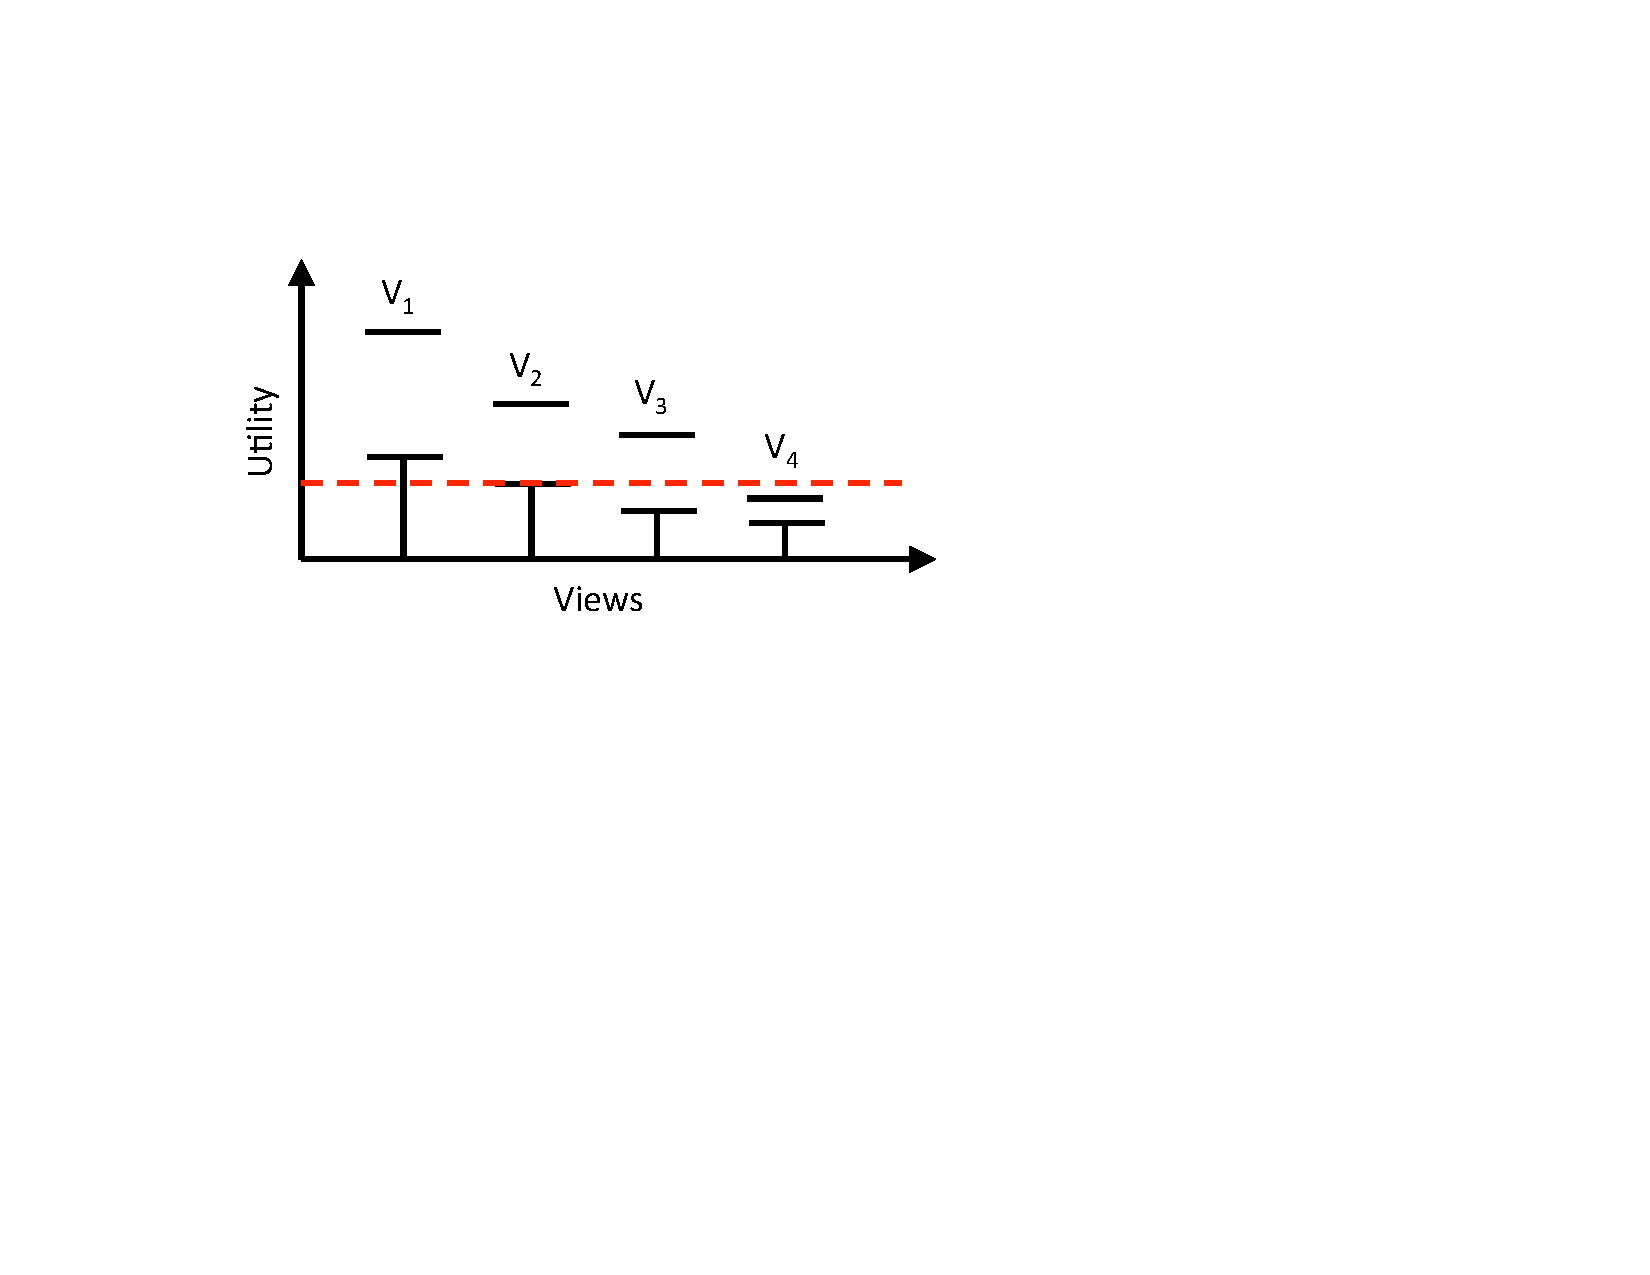
\includegraphics[trim=10mm 100mm 55mm 35mm, 
clip=true]{Images/confidence_pruning.pdf}}}}
\vspace{-20pt}
\caption{Confidence Interval based Pruning}
\label{fig:conf_interval}
\vspace{-12pt}
\end{figure}

Suppose at the end of phase $p$, confidence intervals for the views in
running have values shown in Figure \ref{fig:conf_interval} and we want to
identify the two views with the highest utility.
Views $V_1$ and $V_2$ have the highest utilities so far.
Consider view $V_3$; we see that its confidence interval overlaps with the
confidence intervals of the current top views $V_1$ and $V_2$, making it possible
that $V_3$ will be in the final top views. On the other hand, the confidence
interval for $V_4$ lies entirely below the lowerbounds of $V_1$ and $V_2$.
Since we can claim with high probability (depending on the confidence threshold)
that the utility of $V_4$ lies within its confidence interval, it follows that
with high probability, $V_4$'s utility will be lower than that of both $V_1$ and
$V_2$, and it will not appear in the top-$2$ views.
This is essentially our pruning rule. 

Next, we discuss the two techniques we support to compute confidence intervals.


\stitle{Worst-Case Confidence Intervals.} 
Suppose we have $N$ values $y_1, \ldots, y_n$ in $[0, 1]$, and we are drawing
from them without replacement. 
Say we have drawn $m$ values so far, which are $Y_1, \ldots, Y_m$.
Then, we use the Hoeffding-Serfling inequality~\cite{serfling1974probability} 
to derive a running 
confidence interval around the current mean 
of the $m$ values such that the actual mean of the $N$
is always within this confidence interval with a probability of $1 - \delta$:
\begin{theorem}
\label{thm:hs}
Let $\calY = y_1,$ $\ldots,$ $y_N$ be a set of $N$ 
values in $[0,1]$ with average value
$\frac1N \sum_{i=1}^N y_i = \mu$.
Let $Y_1,\ldots,Y_N$ be a 
sequence of random variables drawn from $\calY$ without
replacement.
Fix any $\delta > 0$. For $1 \le m \le N-1$, define
$$
\varepsilon_m = \sqrt{\frac{(1-\frac{m-1}N)(2\log \log (m) + \log(\pi^2/3\delta))}{2m}}.
$$
$$
\textrm{Then:} \ \   \Pr\left[ \exists m, 1 \le m \le N : 
  \left|\frac{\sum_{i=1}^m Y_i}{m} - \mu\right| > \varepsilon_m \right] 
\le \delta.
$$
\end{theorem}
In our setting, we treat the current mean, $\sum Y_i / m$ is the 
the current estimate of the utility of a view 
based on the entire set of records seen thus far that apply to that view. 
Therefore, to apply this pruning strategy, the only statistics
we need are the current estimate of the utilities.

Note that in this setting, we are assuming that since the
utility estimate at any stage of processing is in $[0, 1]$, 
the $Y_i$ values, i.e., the incremental contributions to the utility
that come from reading each record, are also between $[0, 1]$,
and are independent of the current value of the utility. 
This is is not true in our setting, 
because the utility function could be arbitrary.
Thus, the guarantees do not directly apply to our setting. 

\stitle{Normal Confidence Intervals.} In this scheme,
we apply the standard normal confidence intervals to our utility measurements
assuming that the underlying distribution is Gaussian.
% We describe the equations first assuming that
% when every time a record is read, for every view,
% a utility value is ``sampled''
% from a normal distribution. (This assumption is not
% quite correct; we will discuss this  below.)

Consider a specific view $V_i$. 
If the mean utility across the sampled records 
(i.e., the records read thus far) is $\mu$,
and the variance in the utility of the sampled records
is $\sigma$, then, we have:
\begin{align}
CI & = \mu \pm z \times \frac{\sigma}{\sqrt{m}}
\end{align}
Thus, the CI (or confidence interval) is 
a confidence interval centered around $\mu$, 
and depends on $\sigma$. 
It additionally depends on the number of records
read thus far, $m$,
and $z$, the factor that depends on our confidence interval threshold.
For instance, for a 95\% confidence interval, $z = 1.96$.

We note that the assumption that we are drawing from a normal distribution is
not quite accurate since our samples vary in size and are not independent.
As a result, we make two simple adjustments to the confidence interval
calculations that are described in Appendix \ref{}.
In Section \ref{}, we show experimentally on multiple datasets that our
confidence interval calculations accurately capture utility and can be used to
perform pruning with high confidence.






% \stitle{Normal Confidence Intervals.}
% As described above, we must specify
% a set of statistics to track for each view and a rule that is used to
% prune views based on the statistic.
% For confidence interval based pruning, the statistics we track are the mean, 
% variance, and confidence intervals of the view utility.
% As \VizRecDB\ reads each record, it updates the data
% distributions for all views and calculates the current utility of each view. 
% Using past measures of utility, \VizRecDB\ also tracks the mean,
% variance and confidence intervals for the utility of each view.
% % At the end of a phase, \VizRecDB\ uses the following rule for pruning low-utility
% % views (stated more formally below): {\it if the upperbound on the utility
% % of view $v_i$ is lesser than the least lowerbound on the utility of the
% % top-$k$ views, view $v_i$ is discarded.}

% % Let us dive deeper into this pruning rule.
% Note that as we sequentially read records from a file, we are
% approximating a sampling process (remember that the records are in random order).
% For instance, suppose that we have read 10K records from a 1M record file.
% In this case, the records 1 -- 10K constitute a 1\% sample of the entire file.
% When we read the next say 10 records, the records 1 -- 10,010 constitute an
% incrementally larger sample of the underlying file.
% Thus, as we read more data from the file, we obtaining a large
% number of samples from the underlying data (notice however, that these samples
% are not independent).

% Since we are generating a large number of samples from a population, we can
% invoke a well-studied concept in statistics called the ``sampling distribution.'' 
% A sampling distribution for a statistic $S$ is the distribution of
% $S$ generated by taking a large number of samples of a fixed size and computing
% the statistic $S$ on each sample.
% In our case, the population we draw from is the set of all records in the file
% and our samples are the increasingly larger sets of records that we are reading in.
% The statistic $S$ that we are computing is the view utility (we
% compute a utility value for each view).
% Now, the sampling distribution of the {\it mean} has been well studied and it
% has been proven that the mean of the sampling distribution is equal to the mean of the
% population and the standard error of the sampling distribution is equal to the
% standard error of the population divided by the square root of the sample size. 
% These two formulas are shown in Equations \ref{eq:mean} and \ref{eq:variance}.
% Similarly, if we know the mean and standard error of the sampling distribution,
% we can compute a confidence interval around the population mean. This is shown
% in Equation \ref{eq:confidence_interval} where $z$ is the factor that depends on the
% confidence threshold we are aiming for and $N$ is the number of items
% in each sample.

% \begin{eqnarray}
% \label{eqnarray:mean_and_variance}
% \mu_M = \mu \label{eq:mean}\\
% \sigma_{M} = \frac{\sigma}{\sqrt{N}} \label{eq:variance}\\
% CI = \mu_M \pm z \ast \frac{\sigma_M}{\sqrt{N}}\label{eq:confidence_interval}
% \end{eqnarray}

% If we were modeling the mean of our samples instead of the utility, we could use
% the above result directly.
% However, we find that with a few minor modifications, we can use the confidence
% interval bounds shown above.
% The first modification we make has to do with how we define utility.
% Remember from Section \ref{sec:problem_definition} that the utility of a view is
% defined as the distance between two distributions: the distribution of aggregate values for the
% target view and the distribution of aggregate values for the comparison view.
% These distributions are in turn tied to the number of distinct groups present in
% each dimension attribute.
% For our purposes, it means that if a dimension attribute has $n$ distinct
% groups, then a sample with $x$ rows gives us approximately $\frac{x}{n}$ values
% for each group (assuming uniform distribution).
% Said another way, a sample with $x$ rows for the purpose of computing utility is
% really only a sample of $\frac{x}{n}$ rows.
% So the first modification we make to Equation \ref{eq:confidence_interval} is to
% replace $N$ by $\frac{N}{G_{max}}$ where $G_{max}$ is the maximum number of
% distinct groups present in any dimension attribute.
% Second, we observe that the sampling distribution applies to the case where
% samples are of the same size and are independently generated.
% This is not true in our algorithm; therefore, to compensate, make two
% conservative modifications: we set $N$ to the number of rows that
% have been read in the previous phase (remember that pruning happens at the end
% of every phase) and we set the $z$ parameter to a value $\geq$ 1.96 (the normal
% 95\% confidence interval value). These modifications ensure (as we will show
% empirically in Section \ref{sec:experiments}) that the confidence intervals
% always contain the mean and continually shrink as we read in more data.

% As shown in Line 12 of Algorithm \ref{algo:custom_exec_engine},
% when a phase ends, we clear all statistics collected in that phase; we do not
% want less accurate estimates from previous phases to contaminate the more
% accurate estimates from subsequent phases. \agp{deal with this.}






% Now that we have a way of finding confidence intervals, we elaborate on how we
% use them to perfom pruning.
% Suppose at the end of phase $p$ the confidence intervals for the views in
% running have values shown in Figure \ref{fig:conf_interval} and we want to
% identify the two views with the highest utility.
% Consider view $V_3$, we see that its confidence interval overlaps with the
% confidence intervals of the current top views $V_1$ and $V_2$, making it likely
% that $V_3$ will be in the final top views. On the other hand, the confidence
% interval for $V_4$ lies entirely below the lowest bound of the top two
% intervals.
% Since we can claim with high probability (depending on the confidence threshold)
% that the utility of $V_4$ lies within its confidence interval, it follows that
% with high probability, $V_4$ will not appear in the top-$2$ views.
% This is essentially our pruning rule. 
% We state the algorithm fomally in
% Algorithm \ref{algo:ci_based_pruning}.

\begin{algorithm}
\caption{Confidence Interval Based Pruning}
\label{algo:ci_based_pruning}
\begin{algorithmic}[1]
\State viewsInRunning.sortByUpperbound()
\State topViews $\gets$ viewsInRunning.getTopK()
\State lowestLowerbound $\gets$ min(lowerbound(topViews))
\For {view $\not \in$ topViews}
\If {view.upperbound < lowestLowerbound}
\State viewsInRunning.remove(view)
\EndIf
\EndFor
\end{algorithmic}
\end{algorithm}

\subsubsection{Multi-Armed Bandit Pruning}
\label{sec:multi_armed_bandit}
The second class of pruning techniques we explore
are based on solutions for Multi-Armed Bandits (MAB), a problem 
in stochastic control. 
The setting is as follows: 
a gambler is faced with several slot
machines (``arms'') that each have an underlying reward
distribution. 
At each turn, the gambler must decide which machine
to play at; when they play the machine, they get a reward.
The gambler needs to decide on a {\em strategy}, i.e.,
which machine to play during every turn, to maximize
eventual, total, or time-decaying rewards~\cite{bandits}.
Recently, variants of MAB have been proposed 
which instead of maximizing total reward, 
focus on finding the bandits with the highest mean reward~\cite{BubeckWV13}.
This is very similar to our setting: each possible view can be thought of as
one arm and our goal is find the views with the highest reward (i.e.
utility).
In MAB, each pull of an arm corresponds to a drawing from a sample
the underlying probability distribution of that arm.
In our case, each new record updates the utilities for every possible view and
the every updated utility can be thought of as a sample from the underlying
utility distribution of that view.
There are two approximations we make here to apply the MAB techniques
to our setting
(as we show in our experimental evaluation,
the approximation works well
for our purposes.): 
(1) although the utility of a
view is ultimately a single value, we can approximate it as a probability
distribution that is normally distributed around the true utility, and 
(2) our running estimate of utility after reading $i$
records is an estimate derived from the above utility distribution.

Algorithm \ref{algo:mab_based_pruning} shows the pruning technique used in the
MAB setting.
This algorithm is an adaptation of Successive Accepts and Rejects
algorithm from \cite{BubeckWV13} for finding the top-$k$ arms with the highest
mean reward.
As before, the processing of the whole file is divided into phases.
% As opposed to the confidence interval technique, we only track a single
% statistic for MAB, namely the utility mean.
At the end of every phase, we adopt the following pruning technique: all views
in running are ranked in order of their utility means. 
We then compute two special differences between the utility means: $\Delta_1$
is the difference between the highest mean and the $k+1$st highest mean, and
$\Delta_n$ is the difference between the lowest mean and the $k$th highest mean.
If $\Delta_1$ is greater than $\Delta_n$, the view with the highest mean is
{\it accepted} as being part of the the top-$k$ (and it no longer participates
in pruning computations).
On the other hand, if $\Delta_n$ is higher, the view with the lowest mean is discarded
from the set of views in the running.


\begin{algorithm}
\caption{MAB Based Pruning}
\label{algo:mab_based_pruning}
\begin{algorithmic}[1]
\State viewsInRunning.sortByUtilityMean()
\State \{$\bar{u}_{i}$\} $\gets$ sorted utility means
\State $\Delta_1$ $\gets$ $\bar{u}_{1}$ - $\bar{u}_{k+1}$
\State $\Delta_n$ $\gets$ $\bar{u}_{k}$ - $\bar{u}_{n}$
\If {$\Delta_1$ < $\Delta_n$}
\State viewsInRunning.acceptTop()
\Else
\State viewsInRunning.discardBottom()
\EndIf
\end{algorithmic}
\end{algorithm}

% \techreport{\cite{BubeckWV13} provides bounds on the optimality of this heuristic for the
% MAB setting.
% Since our problem setup isn't exactly the same, the optimality bounds don't
% transfer directly.
% However, as we show in the experimental section, the MAB heuristic performs well
% on real datasets.}